%----------------------------------------------------------------------------
\appendix
%----------------------------------------------------------------------------
\chapter*{\fuggelek}\addcontentsline{toc}{chapter}{\fuggelek}
\setcounter{chapter}{\appendixnumber}
%\setcounter{equation}{0} % a fofejezet-szamlalo az angol ABC 6. betuje (F) lesz

%\numberwithin{tabular}{section}

\begin{lstlisting}[caption=The Mealy machine seen in Fig.\ref{fig:coffeemealy} in the form of the Xtext the grammar described in Listing \ref{li:xtext}.,label=li:coffeemealy]
MealyMachine{
initialState 
State a states { State a, State b, State c, State d, State e, State dd, State f
}inputAlphabet Alphabet { characters { water , pod , button , clean } }
outputAlphabet Alphabet { characters { done , coffee , none } }
transitions{ 
Transition { input clean output done sourceState a targetState a } , 
Transition { input pod output done sourceState a targetState b } , 
Transition { input water output done sourceState a targetState c } , 
Transition { input button output none sourceState a targetState f } , 
Transition { input pod output done sourceState b targetState b } , 
Transition { input water output done sourceState b targetState d } , 
Transition { input button output none sourceState b targetState f } , 
Transition { input clean output done sourceState b targetState a } , 
Transition { input clean output done sourceState c targetState a } , 
Transition { input pod output done sourceState c targetState dd } , 
Transition { input button output none sourceState c targetState f } , 
Transition { input water output done sourceState c targetState c } , 
Transition { input water output done sourceState d targetState d } , 
Transition { input pod output done sourceState d targetState d } , 
Transition { input clean output done sourceState d targetState a } , 
Transition { input button output coffee sourceState d targetState e } , 
Transition { input water output done sourceState dd targetState dd } , 
Transition { input pod output done sourceState dd targetState dd } , 
Transition { input button output coffee sourceState dd targetState e } , 
Transition { input clean output done sourceState dd targetState a } , 
Transition { input clean output done sourceState e targetState a } , 
Transition { input button output none sourceState e targetState f } , 
Transition { input pod output none sourceState e targetState f } , 
Transition { input water output none sourceState e targetState f } , 
Transition { input clean output none sourceState f targetState f } , 
Transition { input button output none sourceState f targetState f } , 
Transition { input pod output none sourceState f targetState f } , 
Transition { input water output none sourceState f targetState f } } }
\end{lstlisting}

\begin{figure}[H]
	\centering
	\begin{subfigure}{0.5\linewidth}
		\centering
		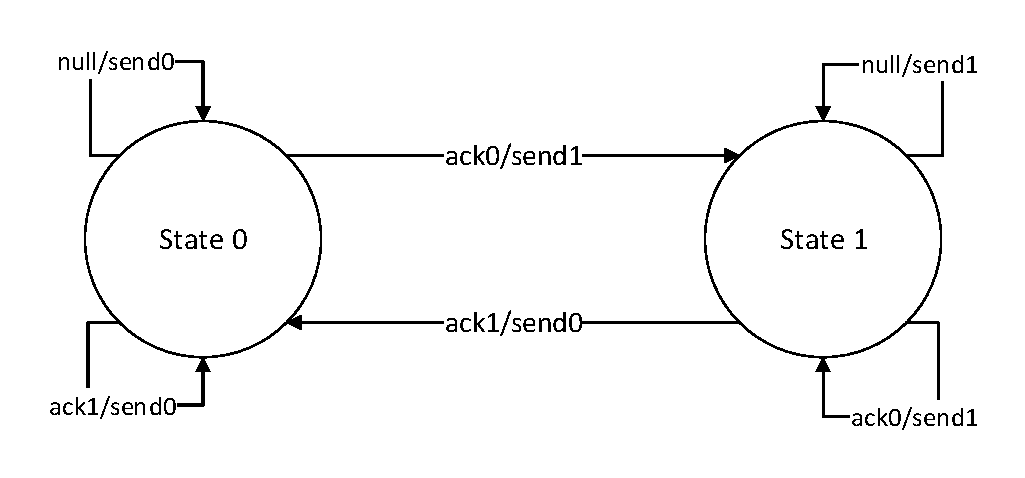
\includegraphics[width=1.0\linewidth]{figures/alternatingbit}
		\caption{Mealy machine representation of the alternating-bit protocol.}
	\end{subfigure}
	\begin{subfigure}{0.8\linewidth}
		\centering
		\begin{lstlisting}
			String sequence = 
				"null|send0|ack1|send0|ack0|send1"
				+ "|ack0null|send1|ack0ack0|send1|ack0ack1|send0"
				+ "|ack1null|send0|ack1ack0|send1|ack1ack1|send0"
				+ "|nullnull|send0|nullack0|send1|nullack1|send0"
				+ "|ack0nullnull|send1|ack0nullack0|send1|ack0nullack1|send0"
				+ "|ack0ack0null|send1|ack0ack0ack0|send1|ack0ack0ack1|send0"
				+ "|ack0ack1null|send0|ack0ack1ack0|send1|ack0ack1ack1|send0"
				+ "|ack1nullnull|send0|ack1nullack0|send1|ack1nullack1|send0"
				+ "|ack1ack0null|send1|ack1ack0ack0|send1|ack1ack0ack1|send0"
				+ "|ack1ack1null|send0|ack1ack1ack0|send1|ack1ack1ack1|send0"
				+ "|nullnullnull|send0|nullnullack0|send1|nullnullack1|send0"
				+ "|nullack0null|send1|nullack0ack0|send1|nullack0ack1|send0"
				+ "|nullack1null|send0|nullack1ack0|send1|nullack1ack1|send0";
		\end{lstlisting}
		\caption{}
	\end{subfigure}
	\caption{A Mealy machine \textbf{(a)}, with its input format \textbf{(b)} using the formalism described in Section \ref{item:stringsequencelearnable}s \emph{StringSequenceLearnable} item.}
	\label{fig:alternatingbit}
\end{figure}


\begin{lstlisting}[caption=Brute-force implementation of equivalence queries described in Section \ref{item:stringsequencelearnable}s \emph{StringSequenceAdapter} item using google guavas Sets.powerSet() function.,label=li:eqbruteforce,float,floatplacement=H]
@Override
public List<? extends I> equivalenceQuery(H hypothesis, Collection<? extends I> alphabet) {
	for(Set<I> s : com.google.common.collect.Sets.powerSet(new HashSet<I>(alphabet))) {
		if(!s.isEmpty()) {
			for(List<I> permutation : com.google.common.collect.Collections2.permutations(s)) {
				if(!hypothesis.query(permutation).equals(this.membershipQuery(permutation))) {
					O a = hypothesis.query(permutation);
					O b = this.membershipQuery(permutation);
					return permutation;
				}
			}
		}
	}
	return null;
}
\end{lstlisting}

\begin{lstlisting}[caption=The output MealyMachine after running the implemented TTT algorithm with the input seen in Listing \ref{li:xtext}.,label=li:xtextttt,float,floatplacement=H]
MealeyMachine{
	initialState State s0
	states {State s0,State s1,State s2,State s3,}
	transitions {
		Transition { input a output top sourceState s0 targetState s1},
		Transition { input b output top sourceState s0 targetState s0},
		Transition { input a output top sourceState s1 targetState s2},
		Transition { input b output top sourceState s1 targetState s1},
		Transition { input a output bot sourceState s2 targetState s3},
		Transition { input b output top sourceState s2 targetState s2},
		Transition { input a output top sourceState s3 targetState s0},
		Transition { input b output bot sourceState s3 targetState s3} }
}
\end{lstlisting}


\begin{lstlisting}[caption=The output MealyMachine after running the implemented DHC algorithm with the input seen in Listing \ref{li:xtext}.,label=li:xtextdhc,float,floatplacement=H]
MealeyMachine{
	initialState State state0
	states {State state0,State state1,State state2,State state3,}
	transitions {
		Transition { input a output top sourceState state0 targetState state1},
		Transition { input b output top sourceState state0 targetState state0},
		Transition { input a output top sourceState state1 targetState state2},
		Transition { input b output top sourceState state1 targetState state1},
		Transition { input a output bot sourceState state2 targetState state3},
		Transition { input b output top sourceState state2 targetState state2},
		Transition { input a output top sourceState state3 targetState state0},
		Transition { input b output bot sourceState state3 targetState state3} }
}
\end{lstlisting}

\begin{lstlisting}[caption=The output MealyMachine after running the implemented DHC algorithm with the input seen in Listing \ref{li:coffeemealy}.,label=li:coffeedhcret,float,floatplacement=H]
MealeyMachine{
	initialState State state0
	states {State state0,State state1,State state2,State state3,State state4,State state5,}
	transitions {
		Transition { input water output done sourceState state0 targetState state1},
		Transition { input pod output done sourceState state0 targetState state2},
		Transition { input button output none sourceState state0 targetState state3},
		Transition { input clean output done sourceState state0 targetState state0},
		Transition { input water output done sourceState state1 targetState state1},
		Transition { input pod output done sourceState state1 targetState state4},
		Transition { input button output none sourceState state1 targetState state3},
		Transition { input clean output done sourceState state1 targetState state0},
		Transition { input water output done sourceState state2 targetState state4},
		Transition { input pod output done sourceState state2 targetState state2},
		Transition { input button output none sourceState state2 targetState state3},
		Transition { input clean output done sourceState state2 targetState state0},
		Transition { input water output none sourceState state3 targetState state3},
		Transition { input pod output none sourceState state3 targetState state3},
		Transition { input button output none sourceState state3 targetState state3},
		Transition { input clean output none sourceState state3 targetState state3},
		Transition { input water output done sourceState state4 targetState state4},
		Transition { input pod output done sourceState state4 targetState state4},
		Transition { input button output coffee sourceState state4 targetState state5},
		Transition { input clean output done sourceState state4 targetState state0},
		Transition { input water output none sourceState state5 targetState state3},
		Transition { input pod output none sourceState state5 targetState state3},
		Transition { input button output none sourceState state5 targetState state3},
		Transition { input clean output done sourceState state5 targetState state0} }
}
\end{lstlisting}

\begin{lstlisting}[caption=The output MealyMachine after running the implemented DHC algorithm with the input seen in Listing \ref{li:coffeemealy}.,label=li:coffeetttret,float,floatplacement=H]
MealeyMachine{
	initialState State s0
	states {State s0,State s1,State s2,State s3,State s4,State s5,}
	transitions {
		Transition { input water output done sourceState s0 targetState s2},
		Transition { input pod output done sourceState s0 targetState s4},
		Transition { input button output none sourceState s0 targetState s1},
		Transition { input clean output done sourceState s0 targetState s0},
		Transition { input water output none sourceState s1 targetState s1},
		Transition { input pod output none sourceState s1 targetState s1},
		Transition { input button output none sourceState s1 targetState s1},
		Transition { input clean output none sourceState s1 targetState s1},
		Transition { input water output done sourceState s2 targetState s2},
		Transition { input pod output done sourceState s2 targetState s3},
		Transition { input button output none sourceState s2 targetState s1},
		Transition { input clean output done sourceState s2 targetState s0},
		Transition { input water output done sourceState s3 targetState s3},
		Transition { input pod output done sourceState s3 targetState s3},
		Transition { input button output coffee sourceState s3 targetState s5},
		Transition { input clean output done sourceState s3 targetState s0},
		Transition { input water output done sourceState s4 targetState s3},
		Transition { input pod output done sourceState s4 targetState s4},
		Transition { input button output none sourceState s4 targetState s1},
		Transition { input clean output done sourceState s4 targetState s0},
		Transition { input water output none sourceState s5 targetState s1},
		Transition { input pod output none sourceState s5 targetState s1},
		Transition { input button output none sourceState s5 targetState s1},
		Transition { input clean output done sourceState s5 targetState s0} }
}
\end{lstlisting}